\section{Task 2}\label{sec:task2}

The goal of the second task is to implement a software to quantify global differences between ensembles and to identify variance along the sequence. The input of this task is a file containing the features of one or more PED ensemble.

\subsection{Ensembles features}
Relationships between different ensambles will be identified considering the structural features of single ensemble using the features file of the task 1.

At the begining, the software extracts the features for each ensamble (multiple conformations):
\begin{itemize}
\item Radius of gyration.
\item Secondary structure entropy for each position acrossensemble conformations
\item Median ASA for each position across ensemble conformations using the model ASA .
\item Median RMSD using rotate-translation matrices for each model.
\item Median distance of each pair of equivalent positions. It consider the matrix columns of conformation distance matrices.
\item Standard deviation of the distance of each pair of equivalent positions.
\end{itemize}


\subsection{Global metric}
The global metric evaluates the distance between ensembles pair. 
The global metric used is.... because....

Using the global metric just described, the software displays the distances between two ensembles through:
\begin{itemize}
\item Heatmap: It calculates the matrix of the distances between the features of the ensambles and then builds and displays the heatmap. In the graph, the distance between ensembles is highlighted with different colors based on the similarity scale on the right. 
\item Dendrogram: Using a linkage matrix and global metric, the distances between pairs of ensembles are evaluated and displayed. The dendrogram combines the most similar ensembles with respect to the calculated features.
\end{itemize}

\begin{figure}[H]
	\begin{minipage}[b]{0.9\textwidth}
		\centering
		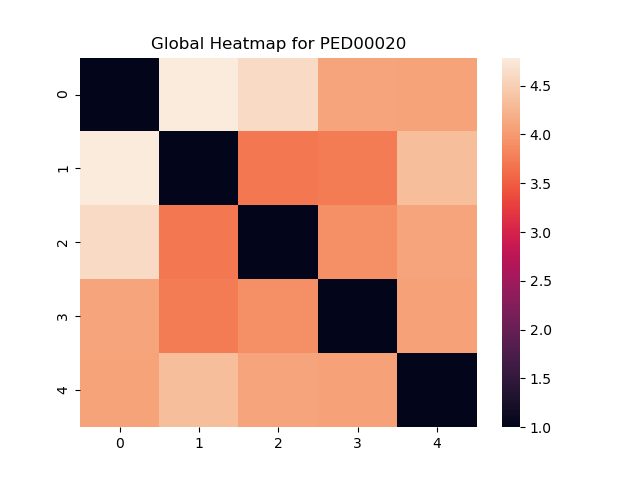
\includegraphics[width=\textwidth]{PED00020_heatmap.png}
		\caption{Heatmap of all the model.}
		\label{heatmap}
	\end{minipage}
	\hfill
	\begin{minipage}[b]{0.9\textwidth}
		\centering
		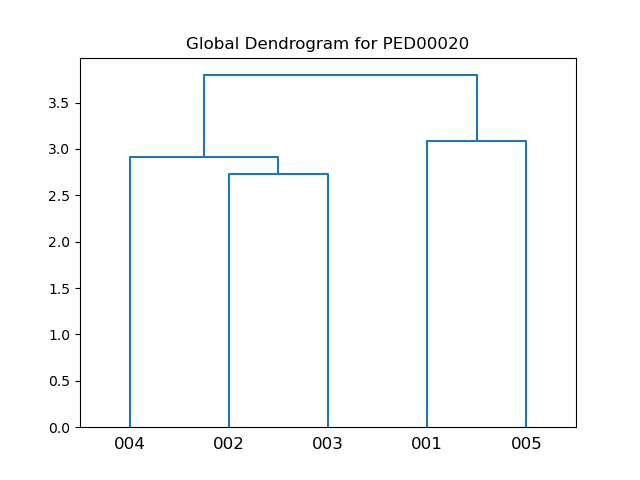
\includegraphics[width=\textwidth]{PED00020_dendrogram.png}
		\caption{Dendrogram of all the model.}
		\label{dendrogram}
	\end{minipage}
\end{figure}

In the previous graphs it is possible to visualize the distance or similarity between the five ensembles within the same PED by comparing the features with the global metric. It can be observed that ensembles 1 and 2 are the most similar (most intense color in the heatmap) and ensemble 4 is the most distant.
We can conclude that... bio


\subsection{Local metric}
The local metric evaluates the variability of all the features for each position in the ensemble.
The local metric used is.... because....

\begin{figure}[H]
	\begin{minipage}[b]{0.9\textwidth}
		\centering
		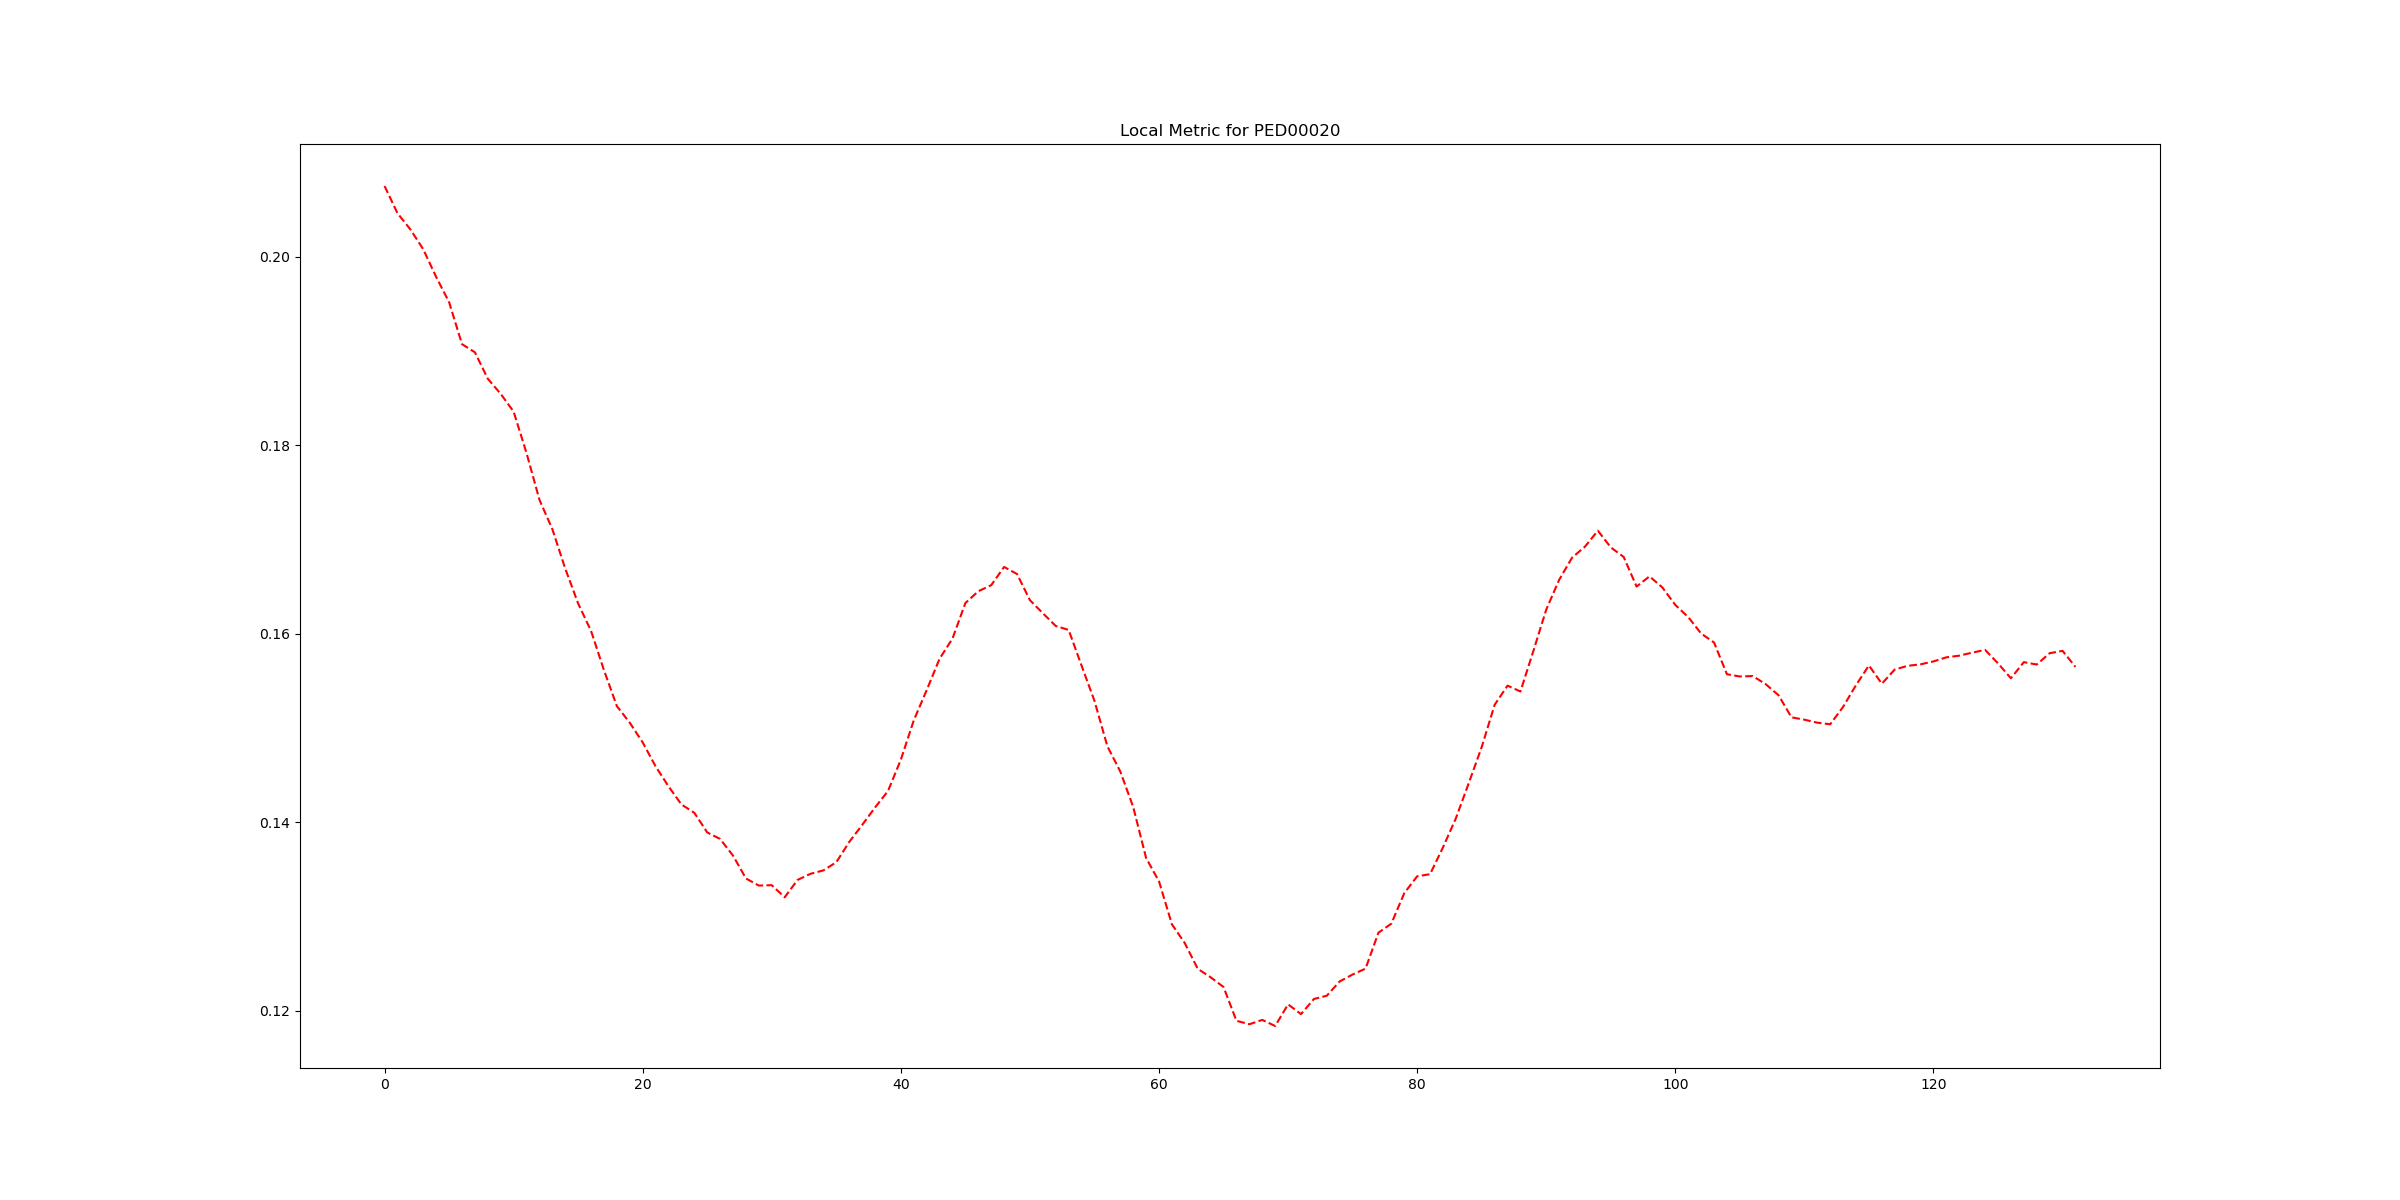
\includegraphics[width=\textwidth]{PED00020_local.png}
		\caption{Plot of local features.}
		\label{plot}
	\end{minipage}	
\end{figure}
In the previous graph it is possible to visualize....it's computed using the local metric that...
We can conclude that... bio